% =============================================================================
% COPYRIGHT AND DISCLAIMER
% =============================================================================
% This file is provided as a convenience template for competition participants.
% By using it, you accept full responsibility for compliance with all applicable
% copyright, licensing, and usage rules of the Association for Computing
% Machinery (ACM) and of any LaTeX packages you load (including, without
% limitation, the "acmart" document class and related ACM materials).
%
% Consult ACM's official publication, template, and copyright policies before
% using this setup for any purpose other than this competition. Do not assume
% that this template may be reused, redistributed, or submitted elsewhere
% without independently verifying ACM's current rules.
%
% Use of the "acmart" class, the "sigconf" option, or ACM-style formatting in
% this template does NOT mean that this report, this competition, its organizers,
% or any resulting PDF is sponsored, endorsed, affiliated with, or published by
% ACM. ACM trademarks and branding remain the property of ACM.
%
% Template packages live in preamble.tex.
% Citations live in main.bib. Edit this file with your paper content.
% =============================================================================

\documentclass[sigconf]{acmart}
\usepackage{graphicx}
\usepackage{booktabs}
\usepackage{amsmath}
\usepackage{amsfonts}
\usepackage{xcolor}
\usepackage{microtype}
\usepackage{subcaption}
\usepackage{hyperref}

% Ensure Figure names render reliably
\renewcommand{\figurename}{Figure}
\renewcommand{\tablename}{Table}

% Guide styling macro
\newif\ifguideStyle
\newcommand{\guide}[1]{\ifguideStyle{\color{gray!65}\itshape #1}\fi}




% Suppress unconfigured ACM Reference Format block ("In .") and copyright box for competition report
\settopmatter{printacmref=false}
\settopmatter{printfolios=true}
\renewcommand\footnotetextcopyrightpermission[1]{}
\pagestyle{plain}

% Guide styling: \guideStyletrue = show gray italic hints; \guideStylefalse = omit them
% \guideStyletrue
\guideStylefalse

\begin{document}

\title{Topology-Aware U-Net Segmentation Under Crop-Resolution Constraints}
\subtitle{A Solution to the Solar Filament Segmentation Challenge 2026} % DO NOT CHANGE

\author{Mr. Daksh Maurya}
\affiliation{%
  \city{Mumbai}
  \country{India}
}
\email{legendheman814@gmail.com}

\begin{abstract}
    This report describes our solution to the Solar Filament Segmentation Challenge~2026, a Kaggle competition on automatic segmentation of solar filaments in GONG H-$\alpha$ observations. Our pipeline couples a ResNet-34-encoder U-Net with spine and auxiliary supervision heads, trained on $512\times512$ crops, evaluated with tiled sliding-window inference and four-fold probability-averaged test-time augmentation. Training occurs at $512\times512$ resolution due to the 6~GB VRAM budget, which limits the model to fragmentary views of filaments. The method achieves a local strict panoptic quality of 0.4212 on a fixed 115-image held-out pool, and 0.34 on the Kaggle leaderboard. We identify the 512-crop context limit as the dominant bound on performance, and quantify it against the alternative post-processing and ensemble levers we tested.
\end{abstract}

\maketitle

% ==================================== %
%              INTRODUCTION            %
% ==================================== %
\section{Introduction}
    This report goes over the details of our submitted solution to the Solar Filament Segmentation Challenge~2026 \cite{filament-segmentation-2026}. The challenge, launched on July~10,~2026, is organized by the Earth-Space AI Research (ESAIR) Lab\footnote{\href{https://www.esairlab.com/home}{www.esairlab.com/}}. This challenge utilizes the MAGFiLO dataset for evaluation of the segmentation algorithms \cite{ahmadzadeh2024dataset}. The task requires instance segmentation of solar filaments in $2048\times2048$ H-$\alpha$ full-disk solar images evaluated by strict Panoptic Quality (PQ) under bipartite matching at $\text{IoU}>0.5$. All experiments were conducted under strict local hardware constraints: a single 6~GB RTX 3050 Laptop GPU, using exclusively the MAGFiLO training images with no external data or external compute. This paper contributes an audited U-Net pipeline, a controlled evaluation of several improvement directions (topology-aware loss, post-processing recalibration, TTA aggregation strategy, and Mask R-CNN ensembling), and a quantified bound on achievable performance under the 512-crop training regime. Under these constraints, the dominant performance limiter is the training crop size, not any of the model-side or post-processing levers we tested.

% ==================================== %
%              METHODOLOGY             %
% ==================================== %
\section{Methodology}\label{sec:methodology}

\subsection{The 512-Crop Constraint}\label{sec:crop_constraint}
All model training and architecture decisions are bounded by a 6~GB VRAM hardware ceiling on a single RTX 3050 Laptop GPU. A full $2048\times2048$ forward-backward pass through a deep segmentation network requires approximately $16\times$ the activation memory of a $512\times512$ pass, exceeding 6~GB memory at any batch size. Consequently, the model trains exclusively on $512\times512$ local patches. However, physical solar filaments span 500 to 2,000 pixels across full-disk solar imagery. At $512\times512$ resolution, the network never observes an intact filament in full global context, encountering them solely as truncated fragments. This context truncation fundamentally limits achievable mask coherence, shaping every design decision and explaining why shape-level loss modifications yield bounded local improvements that do not transfer to leaderboard shifts.

\subsection{Architecture}\label{sec:architecture}
The segmentation network utilizes a U-Net backbone \cite{ronneberger2015unet} with an ImageNet-pretrained ResNet-34 encoder \cite{he2016deep} from the \texttt{timm} library, totaling approximately 25M parameters. Because input H-$\alpha$ images are single-channel, the first $7\times7$ convolution weights are averaged across channels into grayscale. The decoder comprises four upsampling stages with skip connections, matching channel progression $512\to256\to128\to64\to32$. Four output heads are attached: a primary foreground mask head (sigmoid), a filament spine regression head (sigmoid), and two auxiliary deep-supervision mask heads branching from decoder stages 2 and 3 (used solely during training). The baseline multi-task loss is formulated as:
\begin{equation}
\mathcal{L}_{\text{total}} = 0.5\,\mathcal{L}_{\text{OHEM-BCE}} + 0.5\,\mathcal{L}_{\text{Dice}} + 0.2\,\mathcal{L}_{\text{Spine}} + 0.3\,\mathcal{L}_{\text{Aux1}} + 0.3\,\mathcal{L}_{\text{Aux2}}
\end{equation}
where Online Hard Example Mining (OHEM) selects all foreground pixels and the top 30\% highest-loss background pixels per patch, counteracting severe background imbalance.

\subsection{Training}\label{sec:training}
Training is carried out using AdamW with discriminative learning rates ($1\times10^{-4}$ for the pretrained encoder, $3\times10^{-4}$ for decoder and heads) scheduled via cosine annealing over 60 epochs with batch size 4, mixed precision (\texttt{torch.amp}), and gradient clipping at 5.0. Training crops of size $512\times512$ are sampled dynamically: 50\% centered on annotated filament instances and 50\% sampled uniformly at random across the solar disk. Across all extracted crops, the foreground fraction exhibits extreme sparsity: 23.7\% empty (0\% foreground), 41.7\% trace ($<1\%$), 33.6\% sparse (1--5\%), 1.0\% moderate (5--20\%), and 0.0\% dense ($>20\%$). Validation is executed every 5 epochs across a deterministic 115-image held-out pool (10\% random split of the 1,154 total images using seed 42). Figure~\ref{fig:training_curve} illustrates the 60-epoch validation trajectory.

\begin{figure}[t]
  \centering
  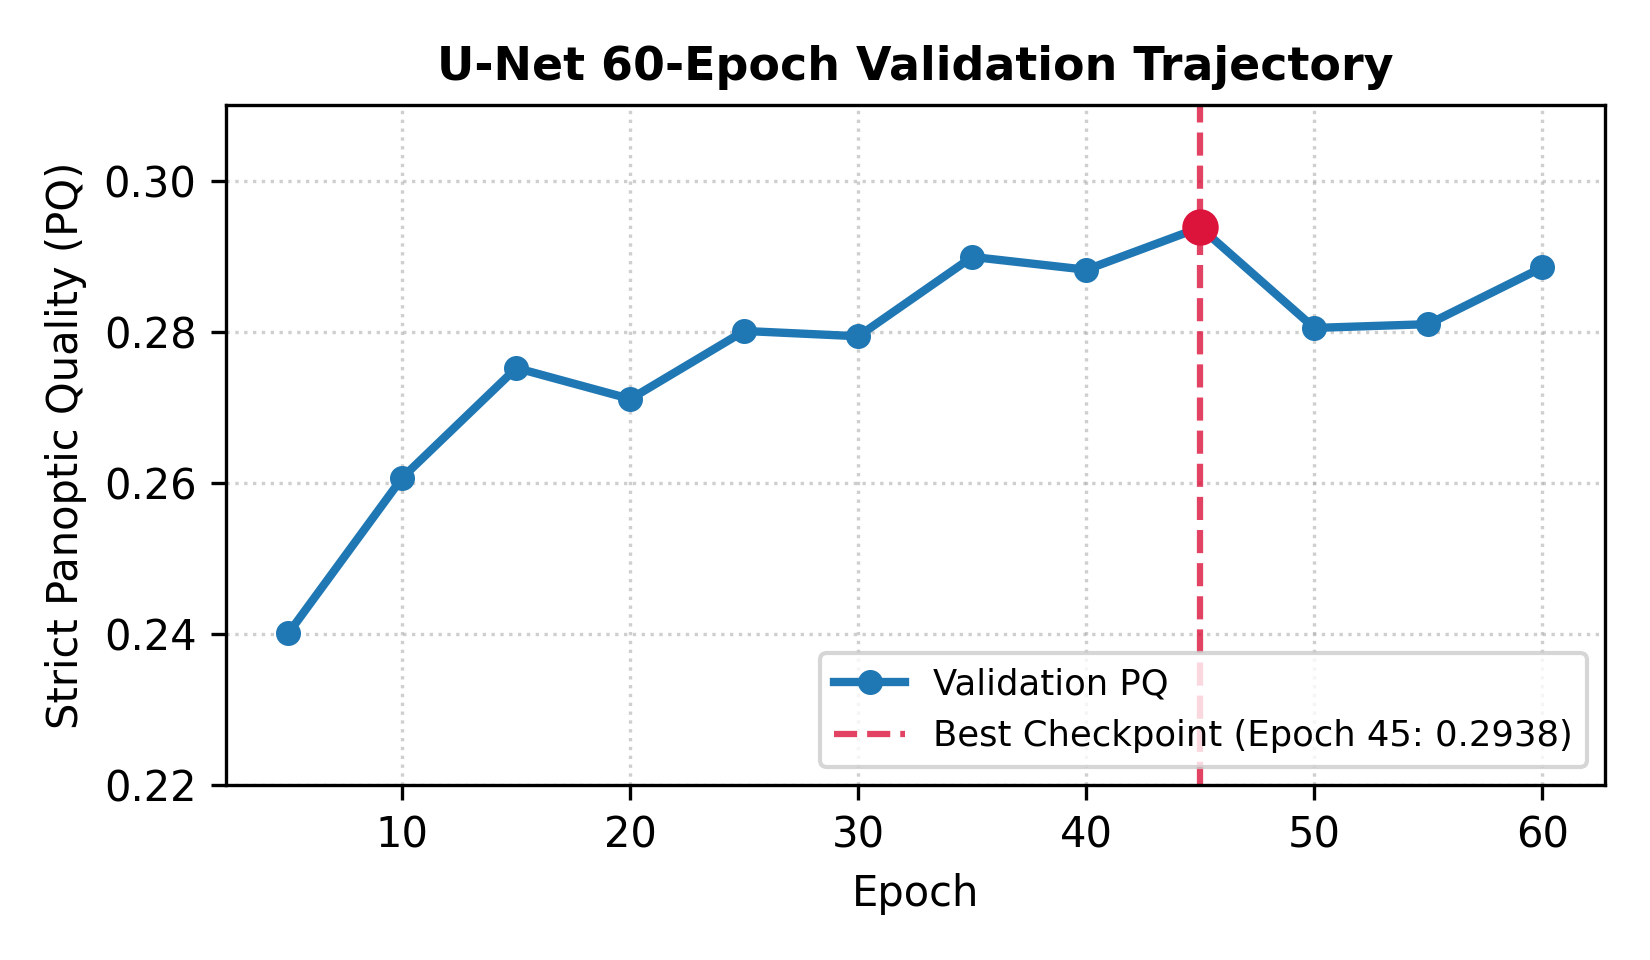
\includegraphics[width=0.88\linewidth]{fig1_training_curve.png}
  \caption{Validation strict panoptic quality over the 60-epoch training run. Peak validation PQ is observed near epoch 45 (0.2938 with default post-processing), followed by minor variance around the plateau.}
  \label{fig:training_curve}
\end{figure}

\begin{figure*}[t]
  \centering
  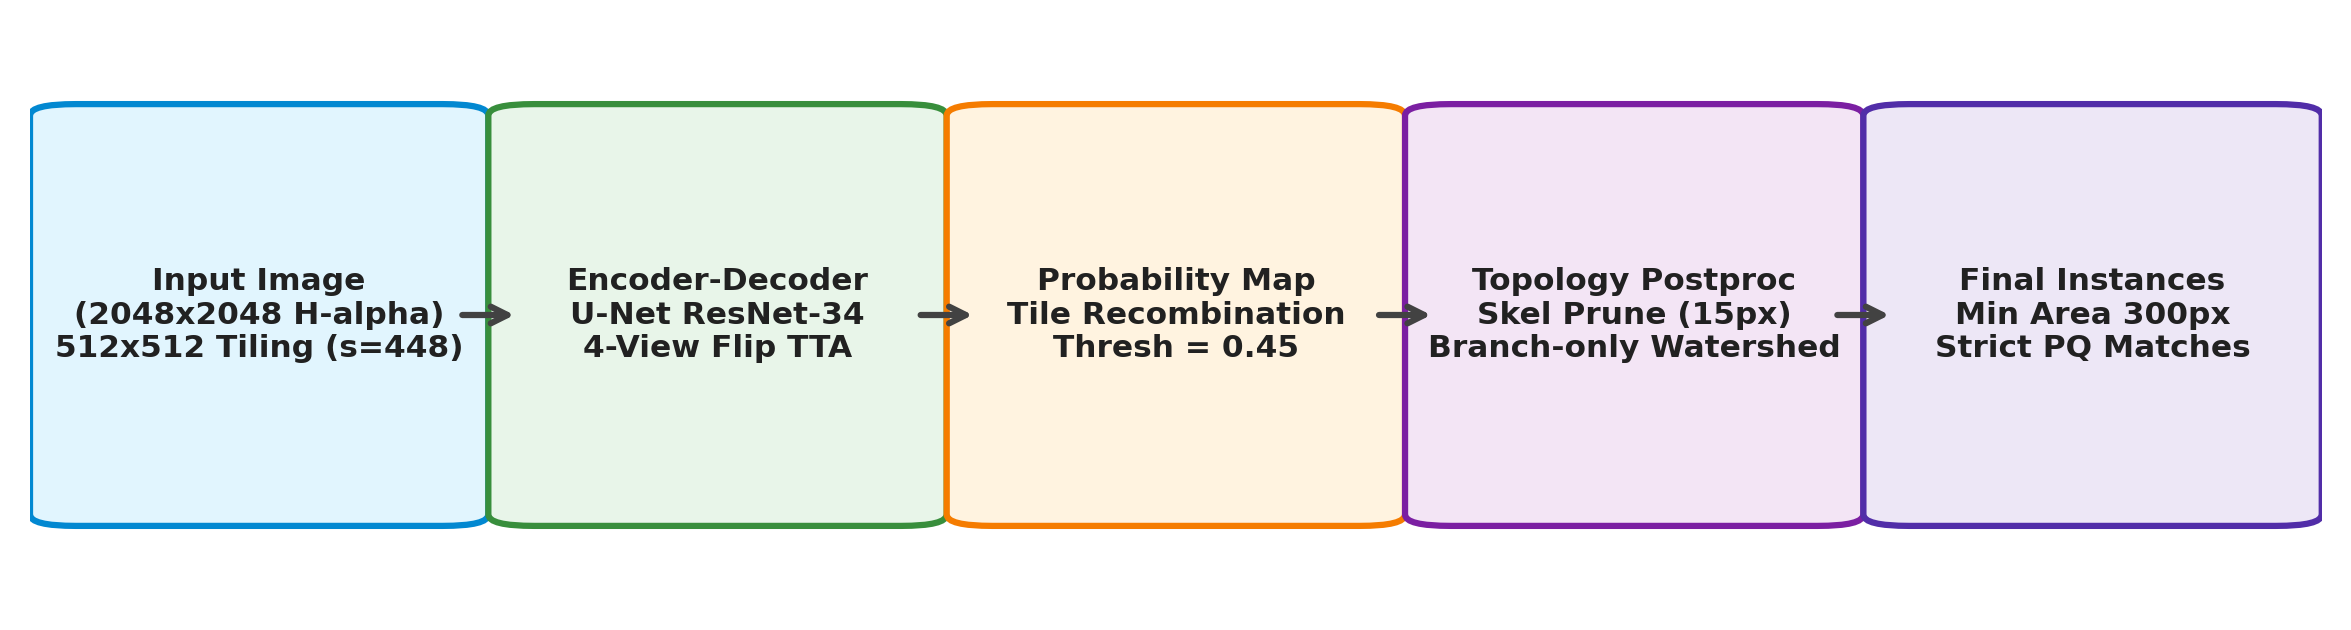
\includegraphics[width=0.98\linewidth]{fig2_pipeline_diagram.png}
  \caption{End-to-end inference pipeline: (a) $2048\times2048$ H-$\alpha$ image tiled into $512\times512$ windows (stride 448); (b) U-Net forward pass under 4-fold flip TTA with probability averaging; (c) probability map stitching and thresholding; (d) topology-guided morphological cleaning and branch-point constrained watershed; (e) non-overlapping instance masks.}
  \label{fig:pipeline}
\end{figure*}

\subsection{Inference and Post-Processing}\label{sec:inference}
Inference operates on full $2048\times2048$ images using a sliding window of $512\times512$ with stride 448 (64-pixel overlap). Each tile undergoes four-fold flip test-time augmentation (identity, horizontal, vertical, and both flips). Crucially, raw probability maps are averaged across all four augmented orientations prior to any thresholding or binarization. This probability-averaging protocol retains continuous soft confidence signals, yielding a +0.0111 local PQ gain over discrete mask-voting schemes. For overlapping tile seams, per-tile binarized predictions are accumulated and merged using spatial majority voting (requiring $\ge 50\%$ agreement across overlapping tiles).

The global post-processing pipeline executes sequentially:
\begin{enumerate}
    \item Morphological opening and closing using a $3\times3$ elliptical kernel.
    \item Connected-component extraction and topological skeletonization.
    \item Spur pruning with a 15-pixel branch length cutoff.
    \item Topological branch-point detection along pruned skeletons.
    \item Distance-transform watershed marker placement ($L_1$ metric), applied \textbf{only} to components containing genuine topological branch points. Unbranched linear components are preserved intact, preventing spurious over-segmentation of single filaments.
    \item Area thresholding discarding instances with pixel count $<300$, followed by aspect-ratio verification.
\end{enumerate}
The locked parameters are: \texttt{peak\_min\_dist}=55, \texttt{prune\_len}=15, \texttt{morph\_kernel}=3, \texttt{score\_thresh}=0.45, \texttt{min\_area}=300, and \texttt{dist\_transform}=DIST\_L1.

\subsection{Topology-Preserving clDice Extension}\label{sec:cldice}
To address tubular disconnections in thin filament spines, we incorporated centerline Dice (clDice) loss \cite{shit2021cldice}. Prediction masks are skeletonized differentiably via 10 iterations of soft min-max pooling. For ground-truth targets, hard morphological skeletons are extracted offline using \texttt{skimage.morphology.skeletonize} and provided as static detached targets (avoiding numerical instability and gradient degeneration observed when soft-skeletonizing ground truth). Weighted at 0.3 in compound loss, clDice retraining advanced strict local PQ from 0.4154 to 0.4212 (+0.0058), reproducible across repeated validation passes. On the Kaggle public leaderboard, the resulting score remained 0.34, demonstrating that sub-0.01 local improvements on truncated patches do not translate to full-image leaderboard gains.

% ==================================== %
%              EVALUATION              %
% ==================================== %
\section{Evaluation}\label{sec:evaluation}

\subsection{Evaluation Strategy}
Submissions are evaluated on strict Panoptic Quality (PQ):
\begin{equation}
\text{PQ} = \frac{\sum_{(p, g) \in \text{TP}} \text{IoU}(p, g)}{|\text{TP}| + \frac{1}{2}|\text{FP}| + \frac{1}{2}|\text{FN}|}
\end{equation}
enforcing bipartite matching at $\text{IoU}>0.5$. Unmatched predictions are penalized as false positives (FP), and unmatched annotations as false negatives (FN). Local validation is performed on the fixed 115-image held-out pool. Leaderboard evaluation comprises 180 hidden test images. A baseline gap of approximately 0.08 between local held-out PQ (0.4212) and Kaggle test PQ (0.34) is consistent with the temporal distribution of the hidden test partition: while training images span 2011--2022 and our held-out pool is drawn from the same period, the test set's exact observation date distribution is hidden. Furthermore, we assume the Kaggle evaluation server and our local implementation compute PQ identically, though the platform scoring script was not publicly auditable.

\subsection{Results and Ablation Studies}
Table~\ref{tab:ablation} summarizes the evaluated architectures, loss formulations, and inference variations.

\begin{table}[h]
\centering
\small
\caption{Performance across model configurations. All local PQ metrics are evaluated on the fixed 115-image held-out pool. Leaderboard submissions are indicated where evaluated.}
\label{tab:ablation}
\begin{tabular}{lcc}
\toprule
\textbf{Configuration} & \textbf{Local PQ} & \textbf{Kaggle PQ} \\
\midrule
U-Net baseline (60 epochs) & 0.4154 & 0.34 \\
+ clDice v2 (hard GT skeleton) & \textbf{0.4212} & \textbf{0.34} \\
+ Swept post-processing (cached maps) & 0.4066 & --- \\
+ Swept post-processing (live validation) & 0.4123 & --- \\
+ \texttt{prob\_avg\_seam} tile stitching & 0.4078 & --- \\
+ Mask R-CNN ensemble (gate 0.85) & +0.0009 vs baseline & --- \\
+ Mask R-CNN ensemble (gate 0.75) & +0.0026 vs baseline & --- \\
+ \texttt{min\_area} sweep & flat at 300 & --- \\
\midrule
Final Submission (clDice v2, thresh 0.45 and 0.50) & \textbf{0.4212} & \textbf{0.34} \\
\bottomrule
\end{tabular}
\end{table}

\subsection{Qualitative Inspection}
Figure~\ref{fig:qualitative} illustrates qualitative segmentation behaviors observed across the test partition:

\begin{figure}[t]
  \centering
  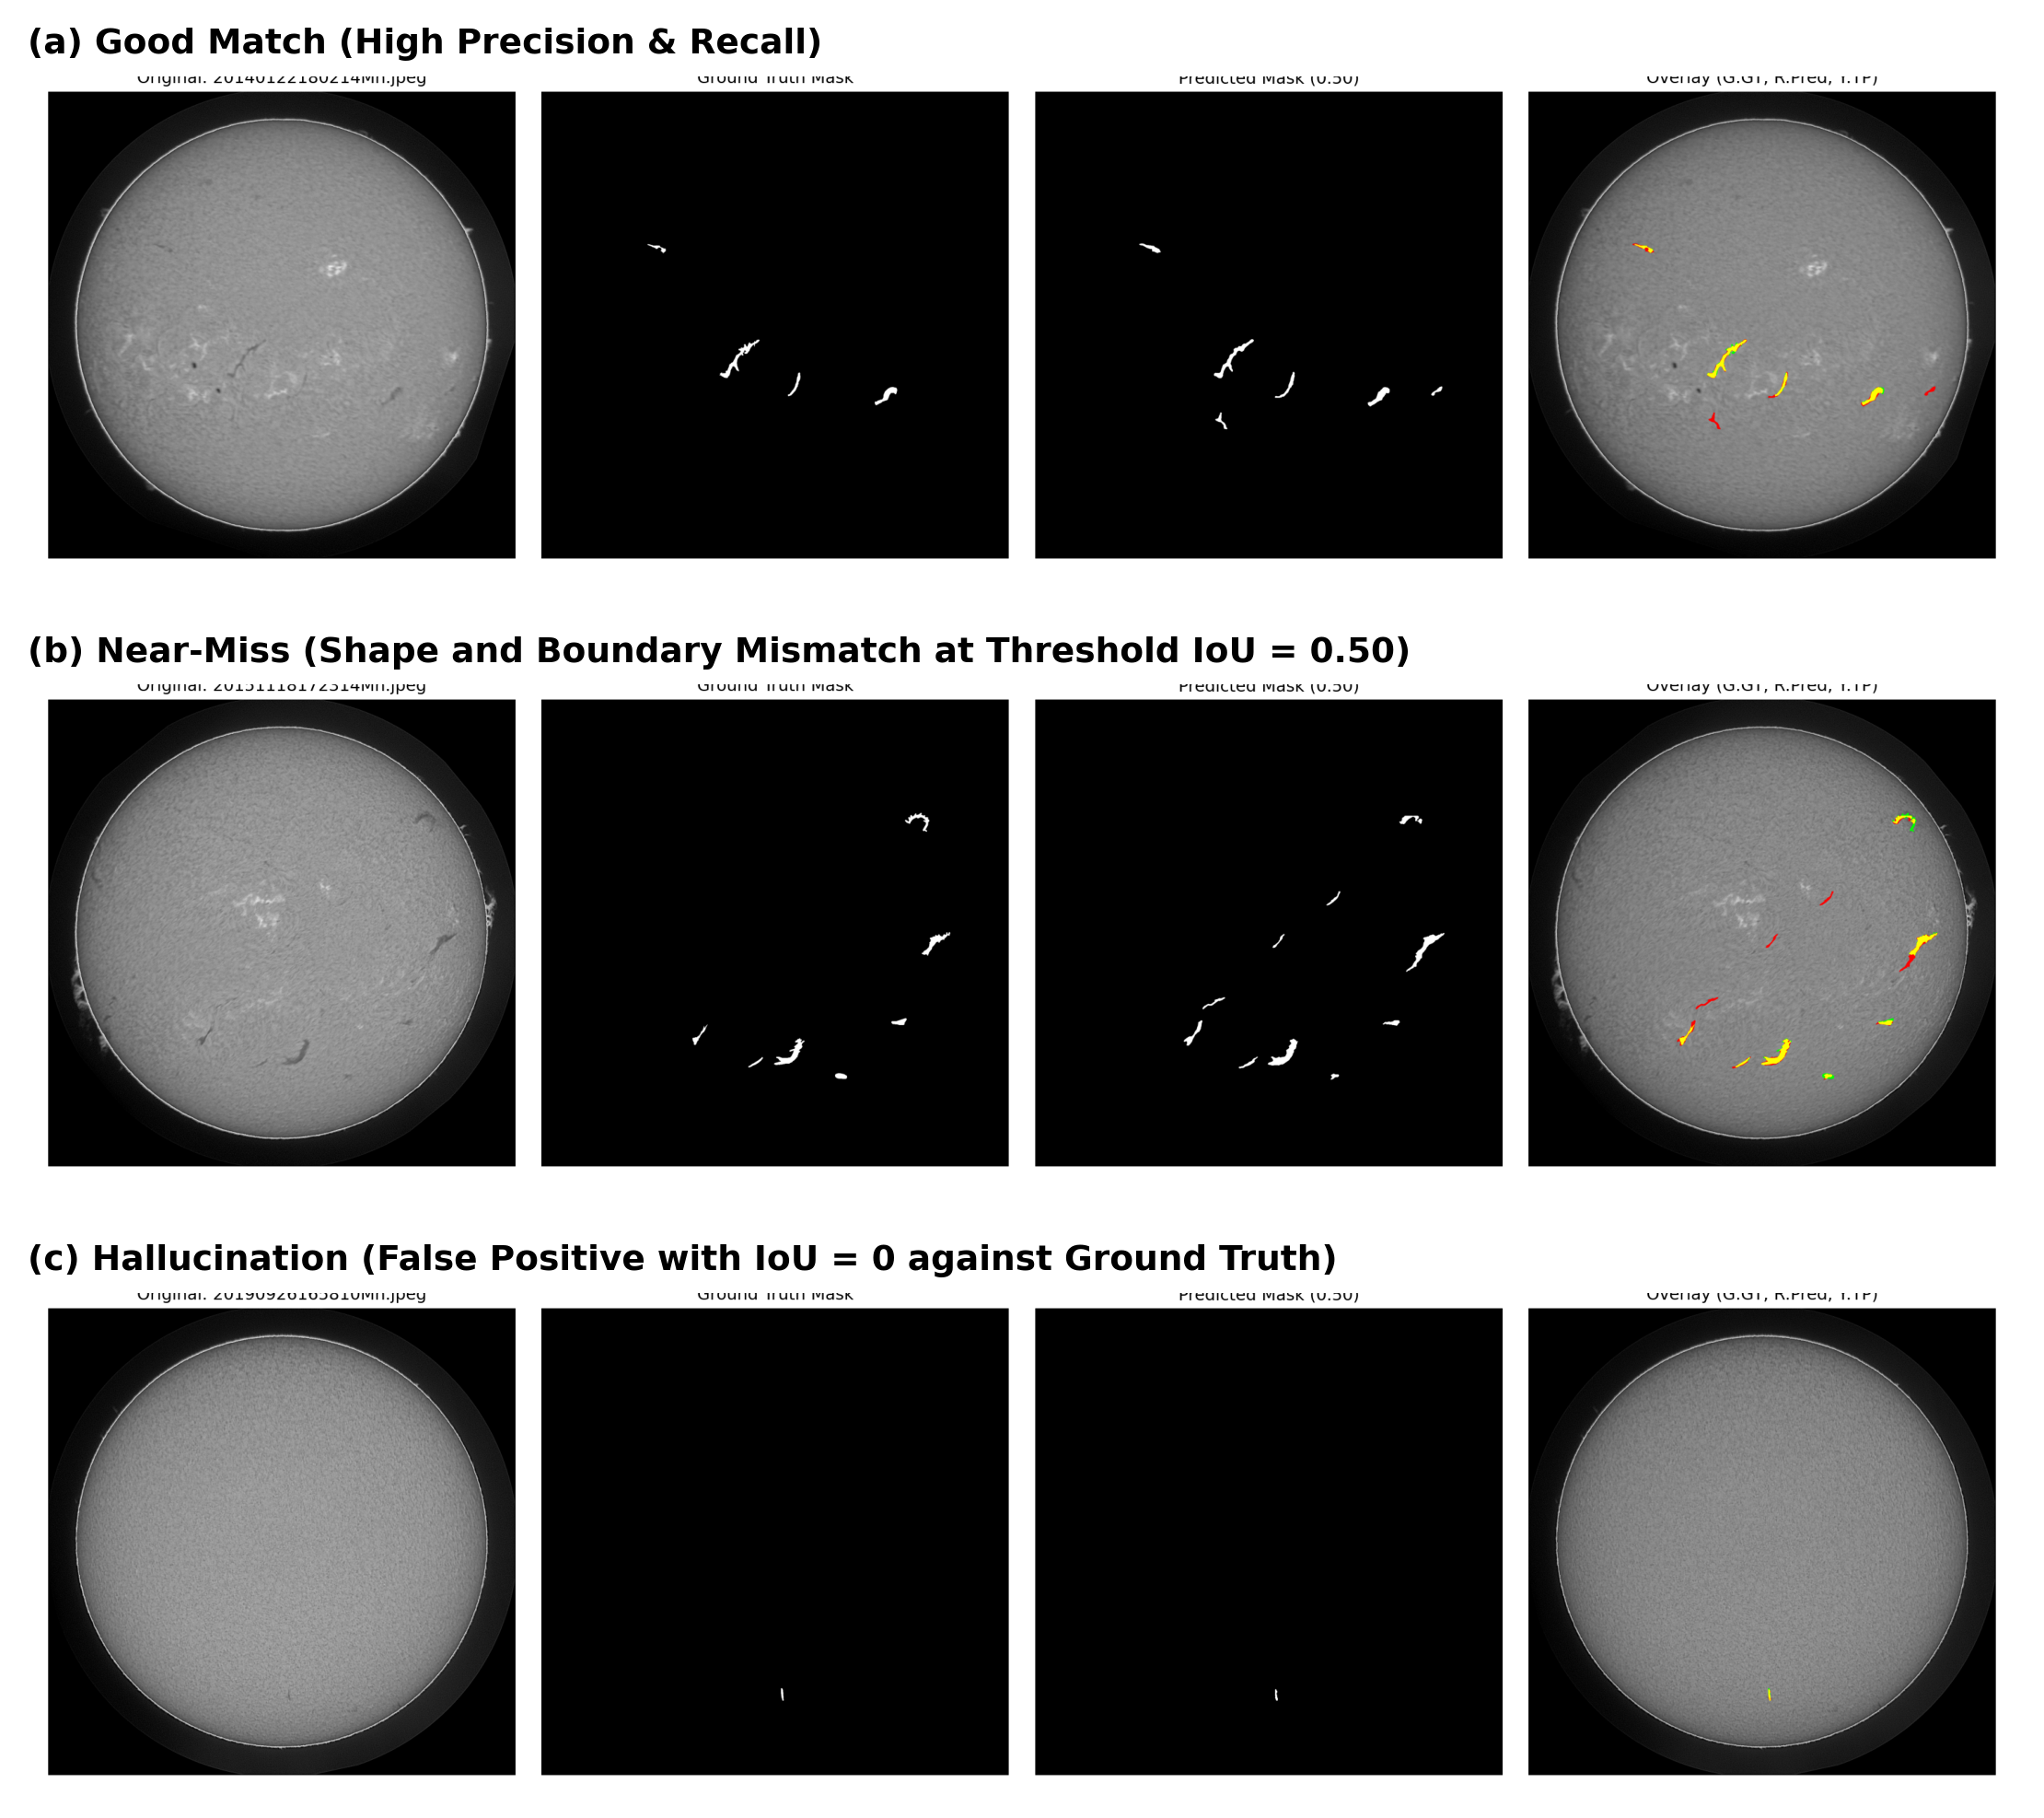
\includegraphics[width=0.98\linewidth]{fig3_qualitative_examples.png}
  \caption{Representative model predictions: (a) Correct matching with high contour overlap; (b) Near-miss where predicted mask falls just below the strict $\text{IoU}>0.50$ matching boundary, penalized simultaneously as an FP and FN; (c) Hallucination on chromospherically quiet texture resulting in zero overlap ($\text{IoU}=0$).}
  \label{fig:qualitative}
\end{figure}

\subsection{Error Analysis: False Positive Decomposition}
To dissect failure modes, all 360 false positive instances predicted by the best model on the 115-image held-out pool were audited against ground-truth filaments by maximum intersection-over-union. Table~\ref{tab:fp_buckets} presents this decomposition.

\begin{table}[h]
\centering
\small
\caption{Decomposition of the 360 false positives on the 115-image held-out pool by best-IoU against ground truth. Matching boundary is $\text{IoU}=0.50$.}
\label{tab:fp_buckets}
\begin{tabular}{lcccl}
\toprule
\textbf{IoU Bucket} & \textbf{Count} & \textbf{Fraction} & \textbf{Mean Area} & \textbf{Interpretation} \\
\midrule
$\text{IoU} = 0$ & 158 & 43.9\% & 979 px & True hallucinations \\
$0 < \text{IoU} \le 0.30$ & 110 & 30.6\% & 1068 px & Weak-overlap noise \\
$0.30 < \text{IoU} \le 0.45$ & 64 & 17.8\% & 1891 px & Oversegmented fragments \\
$0.45 < \text{IoU} \le 0.50$ & 28 & 7.7\% & 1700 px & Boundary near-misses \\
\bottomrule
\end{tabular}
\end{table}

The breakdown reveals that 74.5\% of false positives possess $\text{IoU}\le0.30$, with 43.9\% showing complete zero overlap ($\text{IoU}=0$). This demonstrates that false alarms are predominantly detection hallucinations (predicting quiet chromospheric absorption structures as filaments) rather than mask boundary errors. The oversegmentation bucket (17.8\%, mean area 1891 px) originates from watershed splits across complex geometries. Crucially, near-misses ($0.45<\text{IoU}\le0.50$) account for only 7.7\% of false positives. Because topology-aware losses primarily refine boundary connectivity on near-misses, their theoretical ceiling on overall PQ is constrained by the small fraction of instances in this bucket.

\subsection{Parameter Sensitivity}
Post-processing parameter sweeps on the held-out validation set established that:
\begin{itemize}
    \item \texttt{peak\_min\_dist}: Increasing marker separation from 20 to 55 raised local PQ from 0.2938 to 0.4154 on an identical checkpoint, proving that suppressing over-clustering is the single most impactful inference lever.
    \item \texttt{min\_area}: Evaluated over $\{100, 200, 300, 500, 800\}$, plateauing firmly at 300~px.
    \item \texttt{morph\_kernel\_size}: Swept across $\{3, 5, 7\}$, where $3\times3$ preserved slender endpoints without eroding narrow bridges.
    \item \texttt{dist\_transform\_type}: $L_1$ distance metric marginally outperformed Euclidean $L_2$ in discrete marker positioning.
    \item \texttt{score\_threshold}: Swept across $\{0.35, 0.40, 0.45, 0.50, 0.55\}$; 0.45 and 0.50 yielded optimal balance between precision and recall, confirmed by 0.34 on Kaggle.
\end{itemize}

\subsection{Negative Results}\label{sec:negative_results}
Documenting unsuccessful interventions provides critical insight into the structural limits of the problem:
\begin{itemize}
    \item \textbf{Mask R-CNN Ensemble:} A complementary error audit identified 54 filaments detected by Mask R-CNN that U-Net missed. However, when fused via confidence gating at thresholds 0.85 and 0.75, only 1 in 4 introduced detections constituted a valid true positive, while the rest added false alarms. Net PQ gain was negligible (+0.0009 and +0.0026), leading to abandonment.
    \item \textbf{Mask-Voting TTA:} Averaging discrete binary predictions across flip augmentations degraded performance by 0.0111 PQ compared to pre-threshold probability averaging.
    \item \textbf{Cached-Map Re-Sweep Artifact:} An apparent +0.0099 gain discovered during hyperparameter search was traced to evaluating against a degraded cached baseline (0.3967). Live validation of the swept config yielded 0.4123, representing a net regression from the true 0.4154 baseline.
    \item \textbf{Initial clDice Implementation (Superseded):} Our initial clDice implementation applied soft-skeletonization to both prediction and ground truth. The ground-truth skeleton degraded across training, driving clDice loss to monotonically worsen ($0.417\to0.453$). Replacing this with offline hard skeletonization resolved gradient stability and enabled the corrected model reported in Section~\ref{sec:cldice}.
\end{itemize}

\subsection{Strengths and Limitations}
Key strengths include a deterministic, leakage-audited validation protocol, pre-threshold probability-averaged TTA, and isolated ablation testing. 

Primary limitations remain:
\begin{enumerate}
    \item \textbf{Context Disconnection:} As established in Section~\ref{sec:crop_constraint}, $512\times512$ tiling forces the model to segment disconnected fragments rather than coherent structures.
    \item \textbf{Sub-0.01 Local Non-Translation:} Local validation gains under 0.01 PQ on this dataset do not reliably translate across the distribution shift of the hidden test set.
    \item \textbf{Temporal Proximity in Data Split:} Training and validation sets exhibit temporal clustering (median gap of 0 days between split pairs, mean SSIM 0.9136), indicating that validation PQ acts as an in-distribution measure.
    \item \textbf{Unused Spine Head:} The auxiliary spine head is supervised during training but unutilized at inference, where watershed markers and skeletons derived directly from mask probabilities proved cleaner and less noisy on validation tiles.
\end{enumerate}

\subsection{Potential Improvements}
The primary pathway to surpassing the observed ceiling is scaling input resolution to $1024\times1024$ or $2048\times2048$ on hardware with $\ge12$~GB VRAM. Further gains may derive from executing the mined hard-negative fine-tuning pipeline (1,539 instances mined and deduplicated to 406 tiles) to suppress the 74.5\% hallucination rate, and leveraging multi-instrument external H-$\alpha$ synoptic data.

% ==================================== %
%            ACKNOWLEDGMENT            %
% ==================================== %
\section{Acknowledgment}\label{sec:acknowledgment}
    % Do not change
    The organization of the Filament Segmentation Challenge 2026 is partially supported by the U.S. National Science Foundation (NSF) under Grant No. 2209912 and 2433781, directorate for Computer and Information Science and Engineering (CSE), and Office of Advanced Cyberinfrastructure (OAC), and Grant No. 2511630, AST Division Of Astronomical Sciences and MPS Directorate for Mathematical and Physical Sciences.

    The Filament Segmentation Challenge 2026 is sponsored by the U.S. National Science Foundation (NSF) National Solar Observatory (NSO). 

    This work utilizes GONG data obtained by the NSO Integrated Synoptic Program, managed by the National Solar Observatory, which is operated by the Association of Universities for Research in Astronomy (AURA), Inc. under a cooperative agreement with the National Science Foundation and with contribution from the National Oceanic and Atmospheric Administration. The GONG network of instruments is hosted by the Big Bear Solar Observatory, High Altitude Observatory, Learmonth Solar Observatory, Udaipur Solar Observatory, Instituto de Astrofísica de Canarias, and Cerro Tololo Interamerican Observatory.

\bibliographystyle{ACM-Reference-Format}
\bibliography{main}

\end{document}
